\documentclass[fleqn]{exam}

\usepackage{fullpage}
\usepackage{enumerate}
\usepackage{unitsdef} 
\usepackage{graphicx}
\usepackage[fleqn]{mathtools}
\usepackage{cancel}
\usepackage{polynom}
\usepackage{float}
\usepackage{mdwlist}
\usepackage{booktabs}
\usepackage{cancel}
\usepackage{polynom}
\usepackage{caption}

\setlength{\mathindent}{.5 cm}

\everymath{\displaystyle}

% \begin{figure}[H]
%   \centering
%   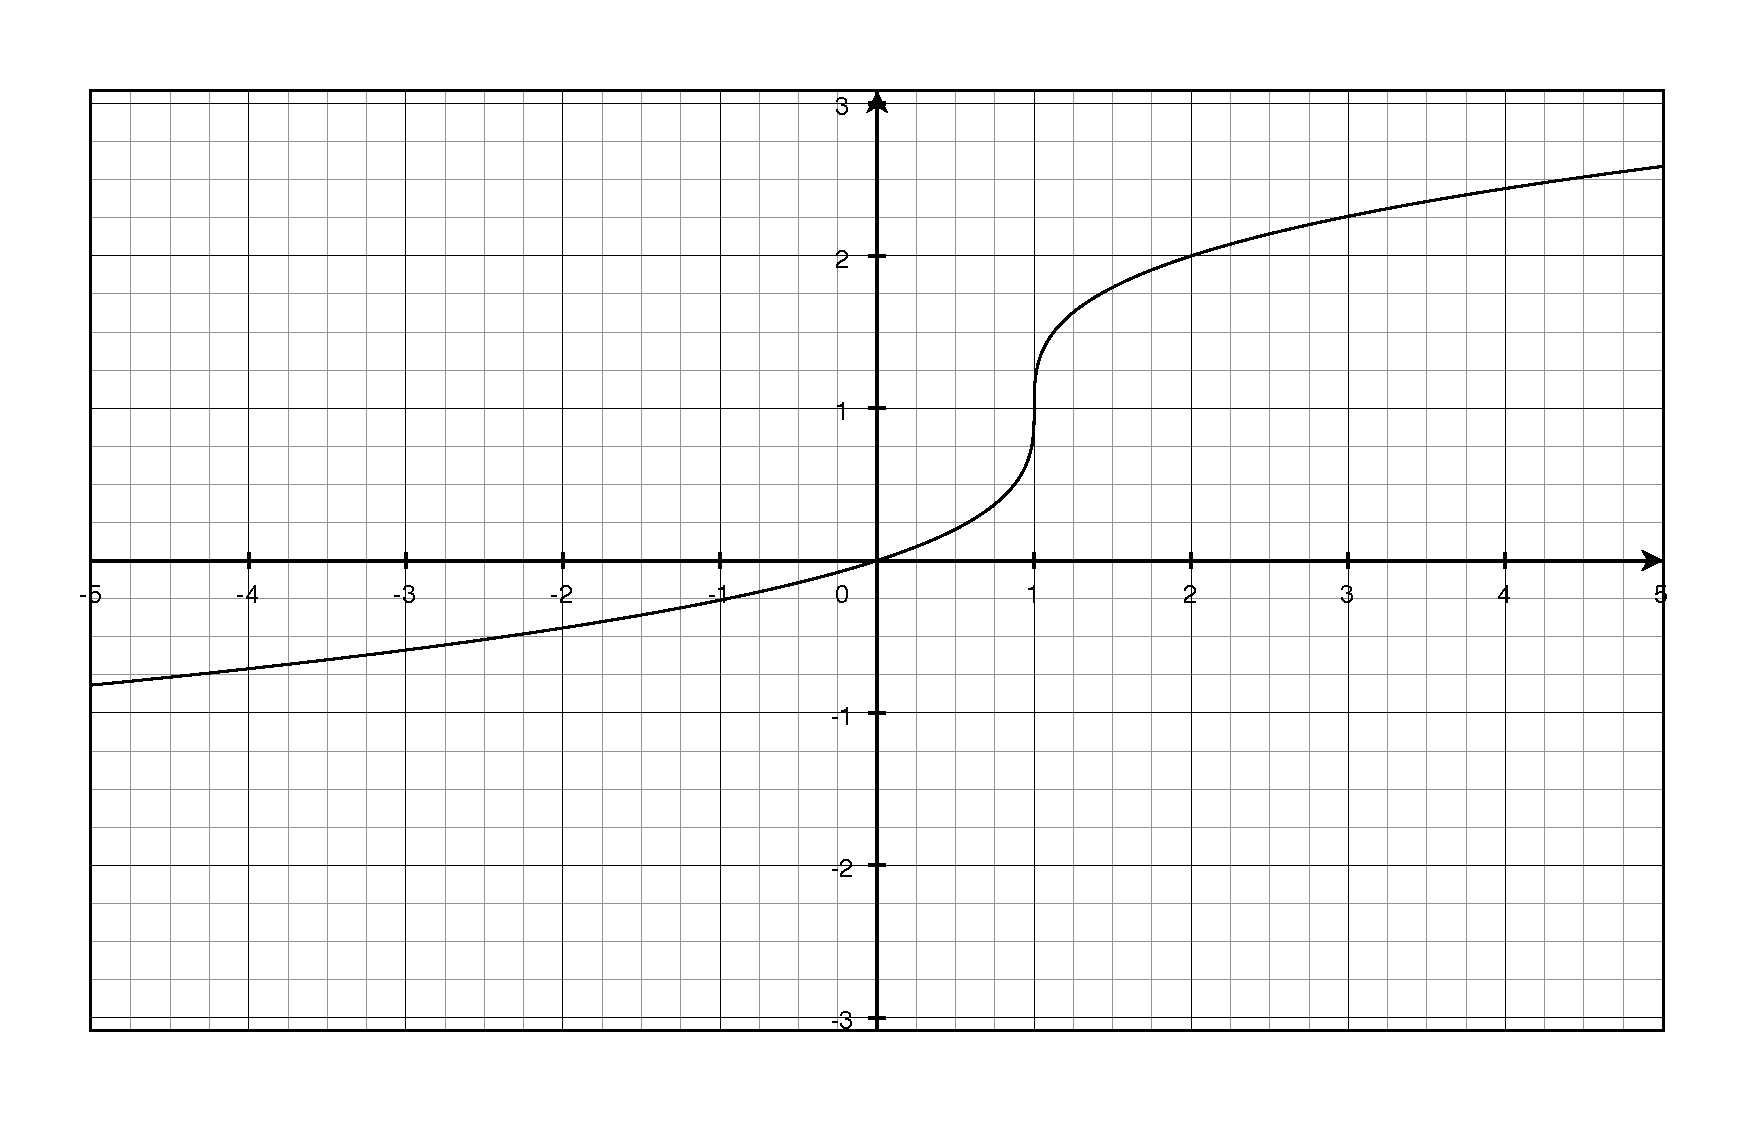
\includegraphics[scale=.3]{question7.eps}
%   \caption*{Question 7}
% \end{figure}

% \begin{tabular}{cc}
% \toprule
% period & amplitude \\
% \midrule
%   $\pi$ & $2$ \\
% \bottomrule
% \end{tabular}

\newunit{\inch}{in}
\newunit{\mile}{mile}
\newunit{\foot}{ft}
\newunit{\knot}{knot}
\newunit{\gallon}{gallon}

\printanswers

\ifprintanswers 
\usepackage{2in1, lscape} 
\fi

\title{Math 263A \\ Homework 16}
\date{May 30, 2012}

\begin{document}

\maketitle

\ifprintanswers
\else
\section{Schedule}

\begin{itemize}
\item Chapter 4 is the last chapter we're covering in this class.  Chapter 5 and beyond is covered in math 263B.

\item The Chapter 4 test will be next week on June 6th.

\item I'm going to be out of town June 13th and June 20th, so there won't be class on those days.  We'll meet again on June
27th to review for the final. 

\end{itemize}

\fi

\section{Homework}

\begin{itemize*}
  \item Read Section 4.7-4.8
  \item pp. 217-220: 2, 3, 9, 12, 16, 28-29, 37, 52
  \item pp. 224-226: 5-10, 13-14, 18-19, 21, 23.  For problems 1-20, you don't need to draw the graph unless you like
    feel you need more practice graphing
\end{itemize*}

\ifprintanswers
\pagebreak
\fi

\section{Extra Credit}
\begin{itemize*}
\item page 225, problem 24
\end{itemize*}

\begin{solution}
\begin{align*}
  f(x) &= \alpha x^2 + \beta x + \gamma \\
  f'(x) &= 2 \alpha x + \beta \\
\\
  rate_{avg} &= \frac{f(b) - f(a)}{b - a} \\
            &= \frac{\alpha b^2 + \beta b + \gamma - (\alpha a^2 + \beta a + \gamma)}{b - a} \\
            &= \frac{\alpha(b^2 - a^2) + \beta(b - a)}{b - a} \\
            &= \frac{\alpha(b + a)(b - a) + \beta(b - a)}{b - a} \\
            &= \frac{(b - a) (\alpha(b + a) + \beta}{b - a} ) \\
            &= \alpha(b + a) + \beta \\
\\
  2 \alpha x + \beta &= \alpha(b + a) + \beta \\
  2 \alpha x &= \alpha(b + a) \\
  x &= \frac{b + a}{2} \\
\end{align*}

\end{solution}

\ifprintanswers
\pagebreak
\fi

%% \section{Review}
%% \begin{questions}

%% \question $D_x\left( \frac{3x^2 + 4}{x^3 - 2x} \right)$

%% \begin{solution}
%% \begin{align*}
%%   D_x\left( \frac{3x^2 + 4}{x^3 - 2x} \right) &= \frac{(x^3 - 2x)(6x) - (3x^2 + 4)(3x^2 - 2)}{(x^3 - 2x)^2} \\
%%   &= \frac{6x^4 - 12x^2 - (9x^4 + 6x^2 - 8)}{(x^3 - 2x)^2} \\
%%   &= \frac{-3x^4 - 18x^2 + 8}{(x^3 - 2x)^2} \\
%% \end{align*}
%% \end{solution}

%% \end{questions}

\ifprintanswers
\pagebreak

\section{Section 4.7}

\begin{description}

\item[2]
\begin{align*}
  f(x)  &= 2x^3 - 3x - 10 \\
  f'(x) &= 6x^2 - 3 \\
  f''(x) &= 12x \\
\end{align*}

Critical Points:
\begin{align*}
  6x^2 - 3 &= 0 \\
  2x^2 - 1 &= 0 \\
  x &= \pm \sqrt{\frac{1}{2}} \\
\end{align*}

Inflection Points:
\begin{align*}
  12x &= 0 \\
  x &= 0 \\
\end{align*}

\begin{itemize*}
  \item Increasing: $\left(-\infty, -\frac{1}{\sqrt{2}} \right] \cup \left[\frac{1}{\sqrt{2}}, \infty \right)$
  \item Concave up: $(0, \infty)$
\end{itemize*}

\begin{figure}[H]
  \centering
  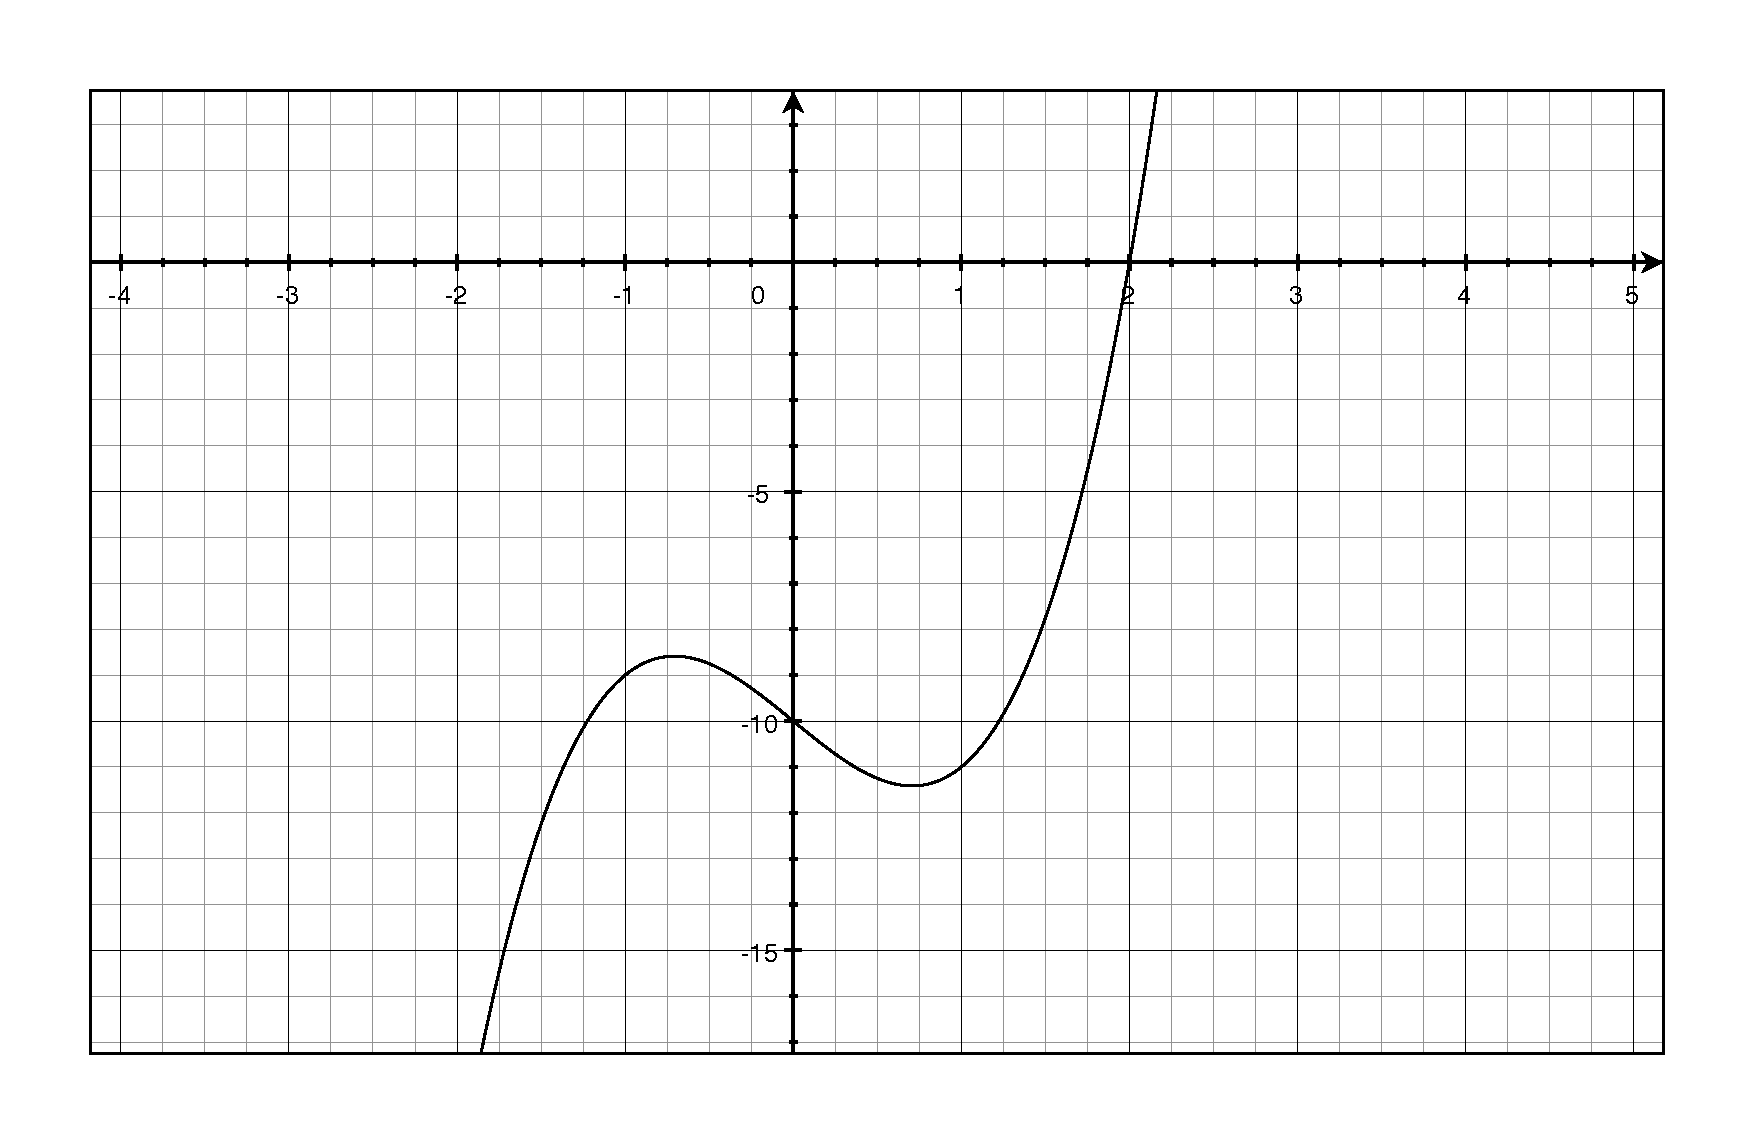
\includegraphics[scale=.3]{4.7.2.eps}
  \caption*{Question 2: $f(x) = 2x^3 - 3x - 10$}
\end{figure}

\pagebreak

\item[3]
\begin{align*}
  f(x) &= 2x^3 - 3x^2 - 12x + 3 \\
  f'(x) &= 6x^2 - 6x - 12 \\
  f''(x) &= 12x - 6 \\
\end{align*}

Critical Points:
\begin{align*}
  6x^2 - 6x - 12 &= 0 \\
  x^2 - x - 2 &= 0 \\
  (x - 2)(x + 1) &= 0 \\
  x &= \{-1, 2\} \\
\end{align*}

Inflection Points:
\begin{align*}
  12x - 6 &= 0 \\
  x &= \frac{1}{2} \\
\end{align*}

\begin{itemize*}
  \item Increasing: $(-\infty, -1] \cup [2, \infty)$
  \item Concave Up: $\left(\frac{1}{2}, \infty \right)$
  \item Vertical Asymptote: $x = -1$
  \item Horizontal Asymptote: $y = 1$
\end{itemize*}

\begin{figure}[H]
  \centering
  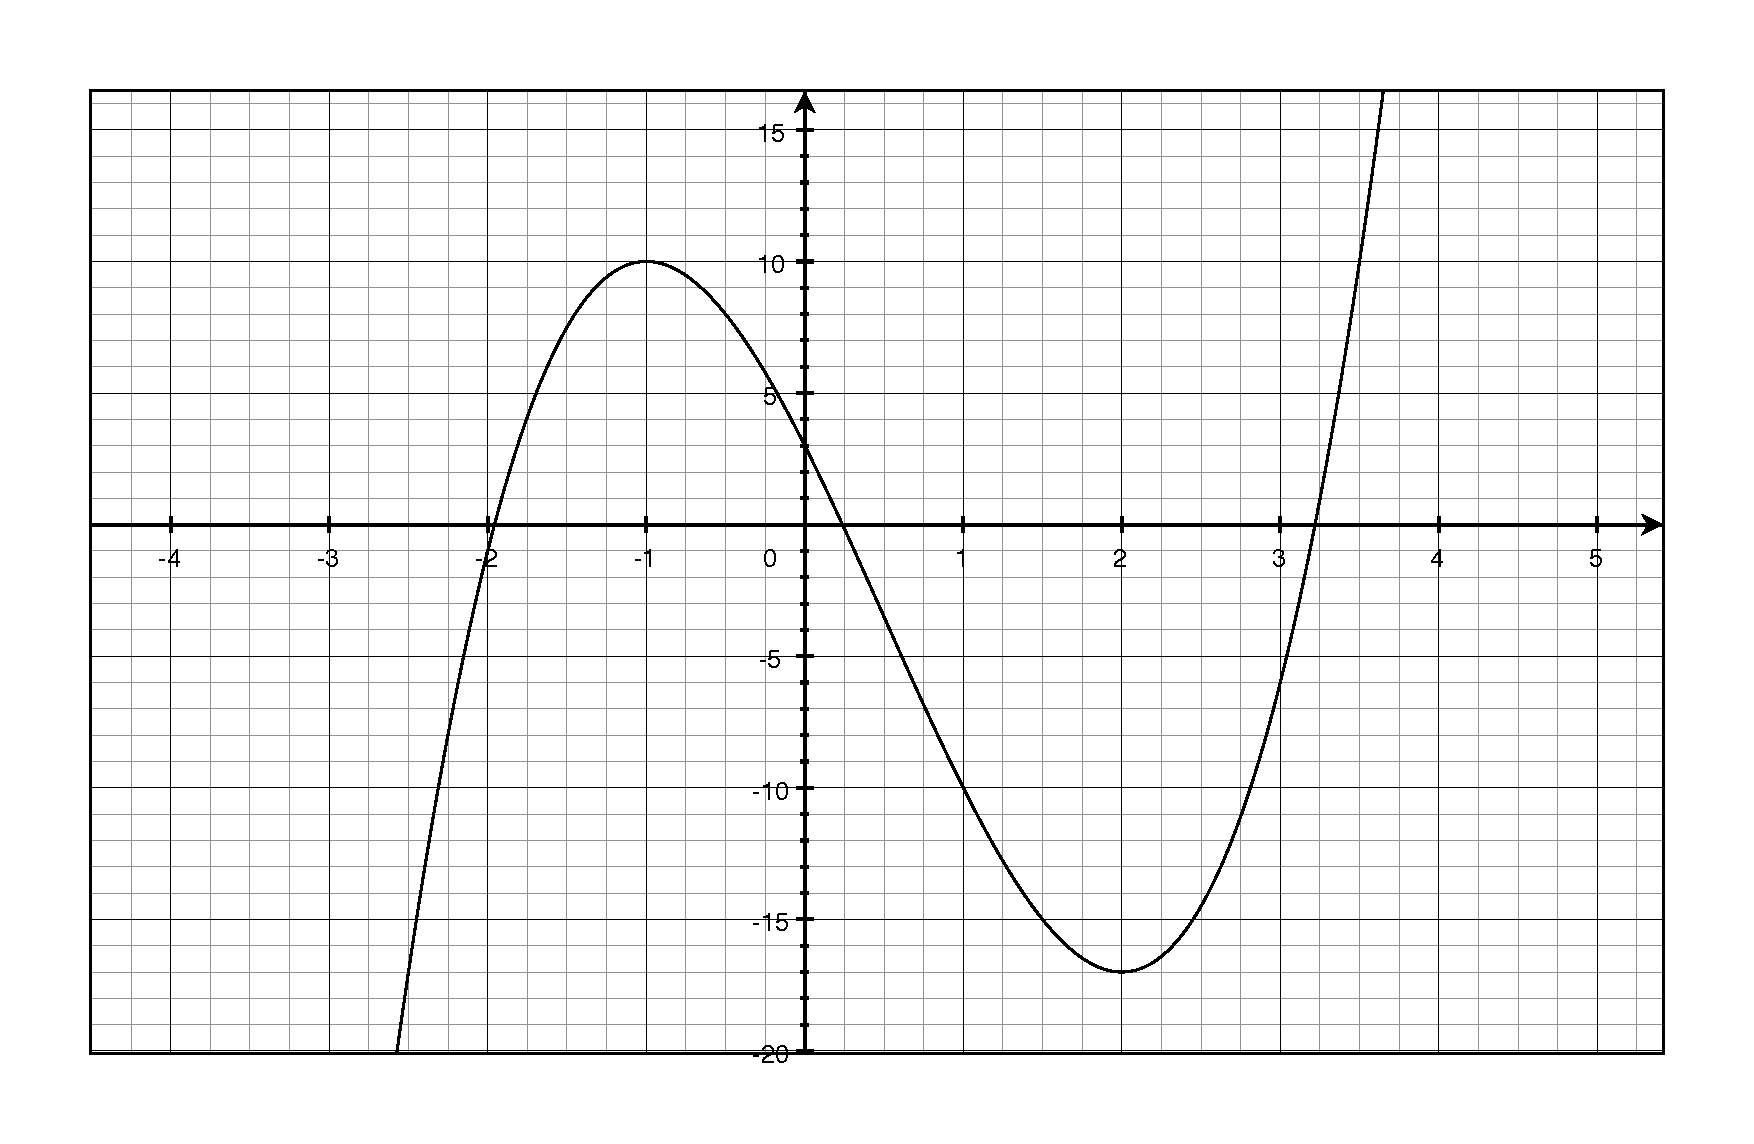
\includegraphics[scale=.3]{4.7.3.eps}
  \caption*{Question 3: $f(x) = 2x^3 - 3x^2 - 12x + 3$}
\end{figure}

\pagebreak

\item[9]
\begin{align*}
  f(x) &= \frac{x}{x + 1} \\
  f'(x) &= \frac{x + 1 - x}{(x + 1)^2} \\
        &= \frac{1}{(x + 1)^2} \\
  f''(x) &= \frac{-2}{(x + 1)^3} \\
\end{align*}

\begin{itemize*}
  \item Increasing: $(-\infty, -1) \cup (-1, \infty)$
  \item Concave up: $(-\infty, -1)$
\end{itemize*}

\begin{figure}[H]
  \centering
  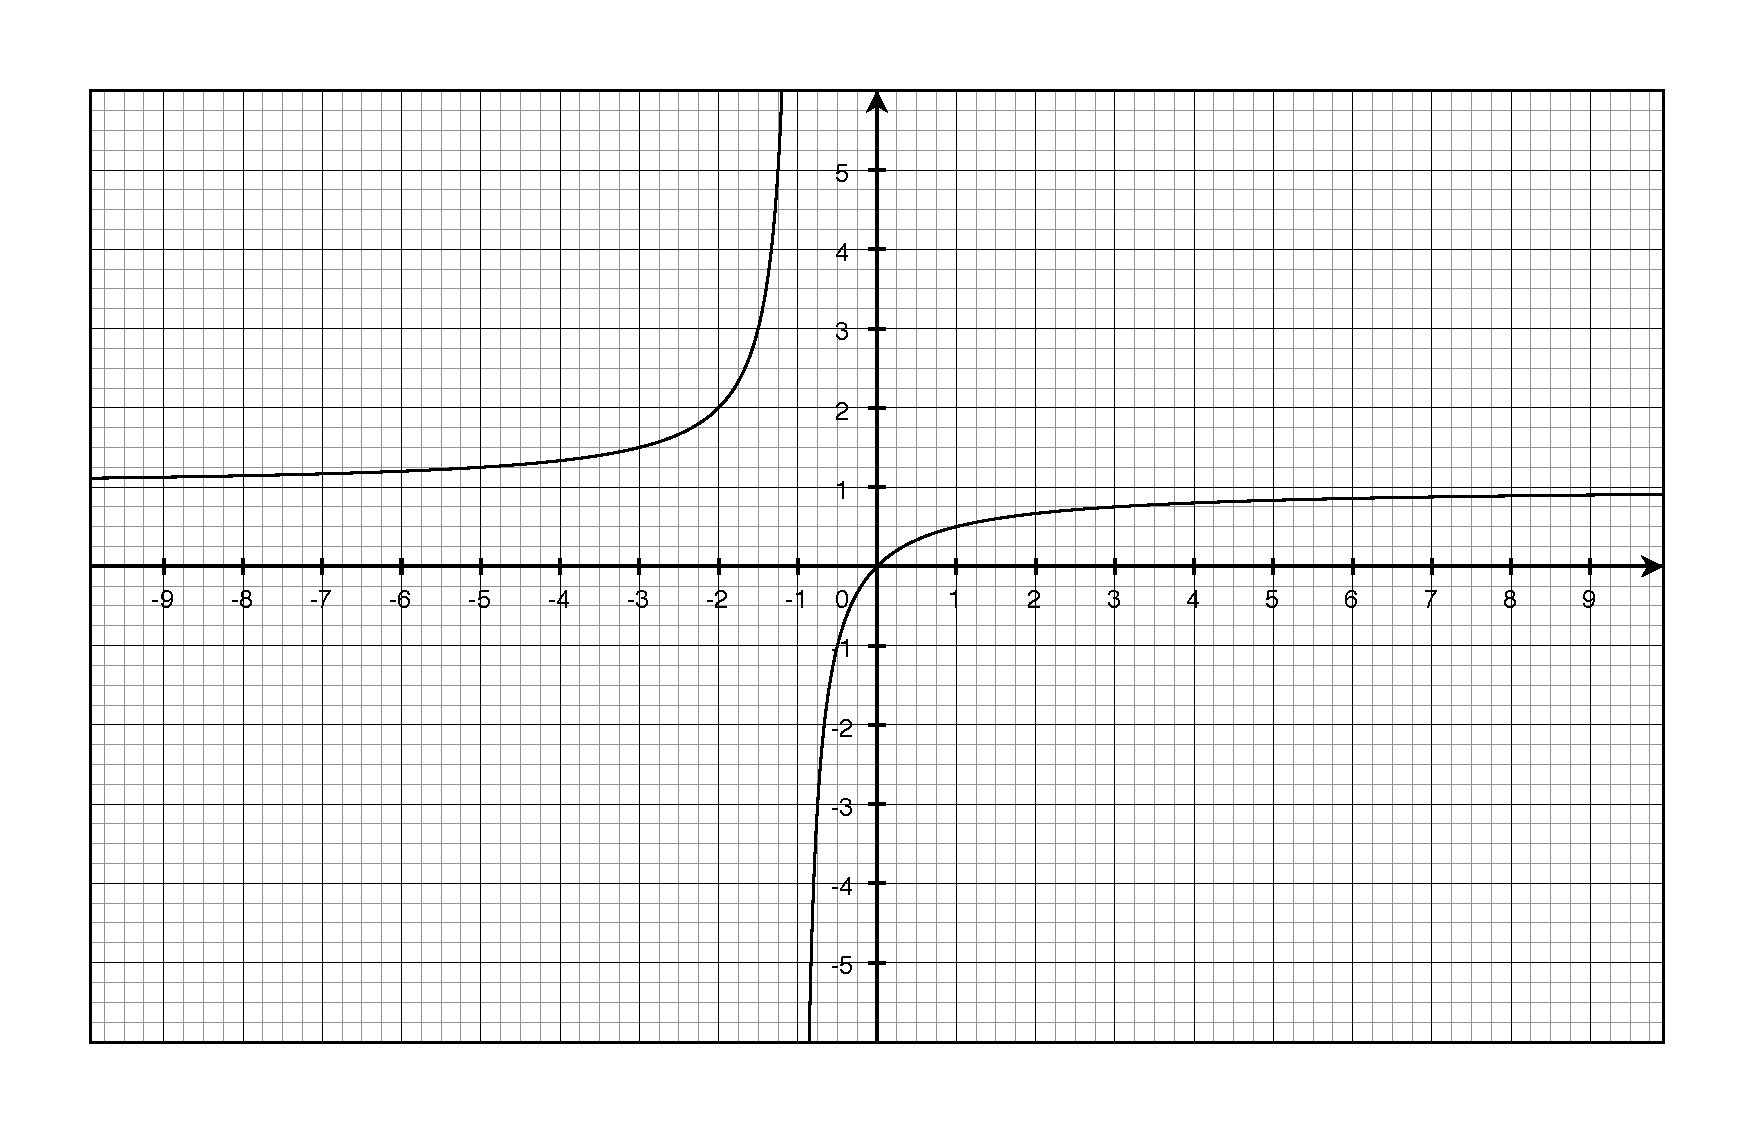
\includegraphics[scale=.3]{4.7.9.eps}
  \caption*{Question 9: $f(x) = \frac{x}{x + 1}$}
\end{figure}

\item[12]
\begin{align*}
  f(\theta) &= \frac{\theta^2}{\theta^2 + 1} \\
  f'(\theta) &= \frac{2 \theta}{(\theta^2 + 1)^2} \\
  f''(\theta) &= \frac{-6 \theta^2 + 2}{(\theta^2 + 1)^3} \\
\end{align*}

Critical Numbers:
\begin{align*}
  \frac{2 \theta}{(\theta^2 + 1)^2} &= 0 \\
  \theta &= 0 \\
\end{align*}

Inflection Points:
\begin{align*}
  \frac{-6 \theta^2 + 2}{(\theta + 1)^3} &= 0 \\
  \theta &= \pm \sqrt{ \frac{1}{3} } \\
\end{align*}

\begin{itemize*}
  \item Increasing: $[0, \infty)$
  \item Concave Up: $\left( -\sqrt{\frac{1}{3}}, \sqrt{\frac{1}{3}} \right)$
\end{itemize*}

\begin{figure}[H]
  \centering
  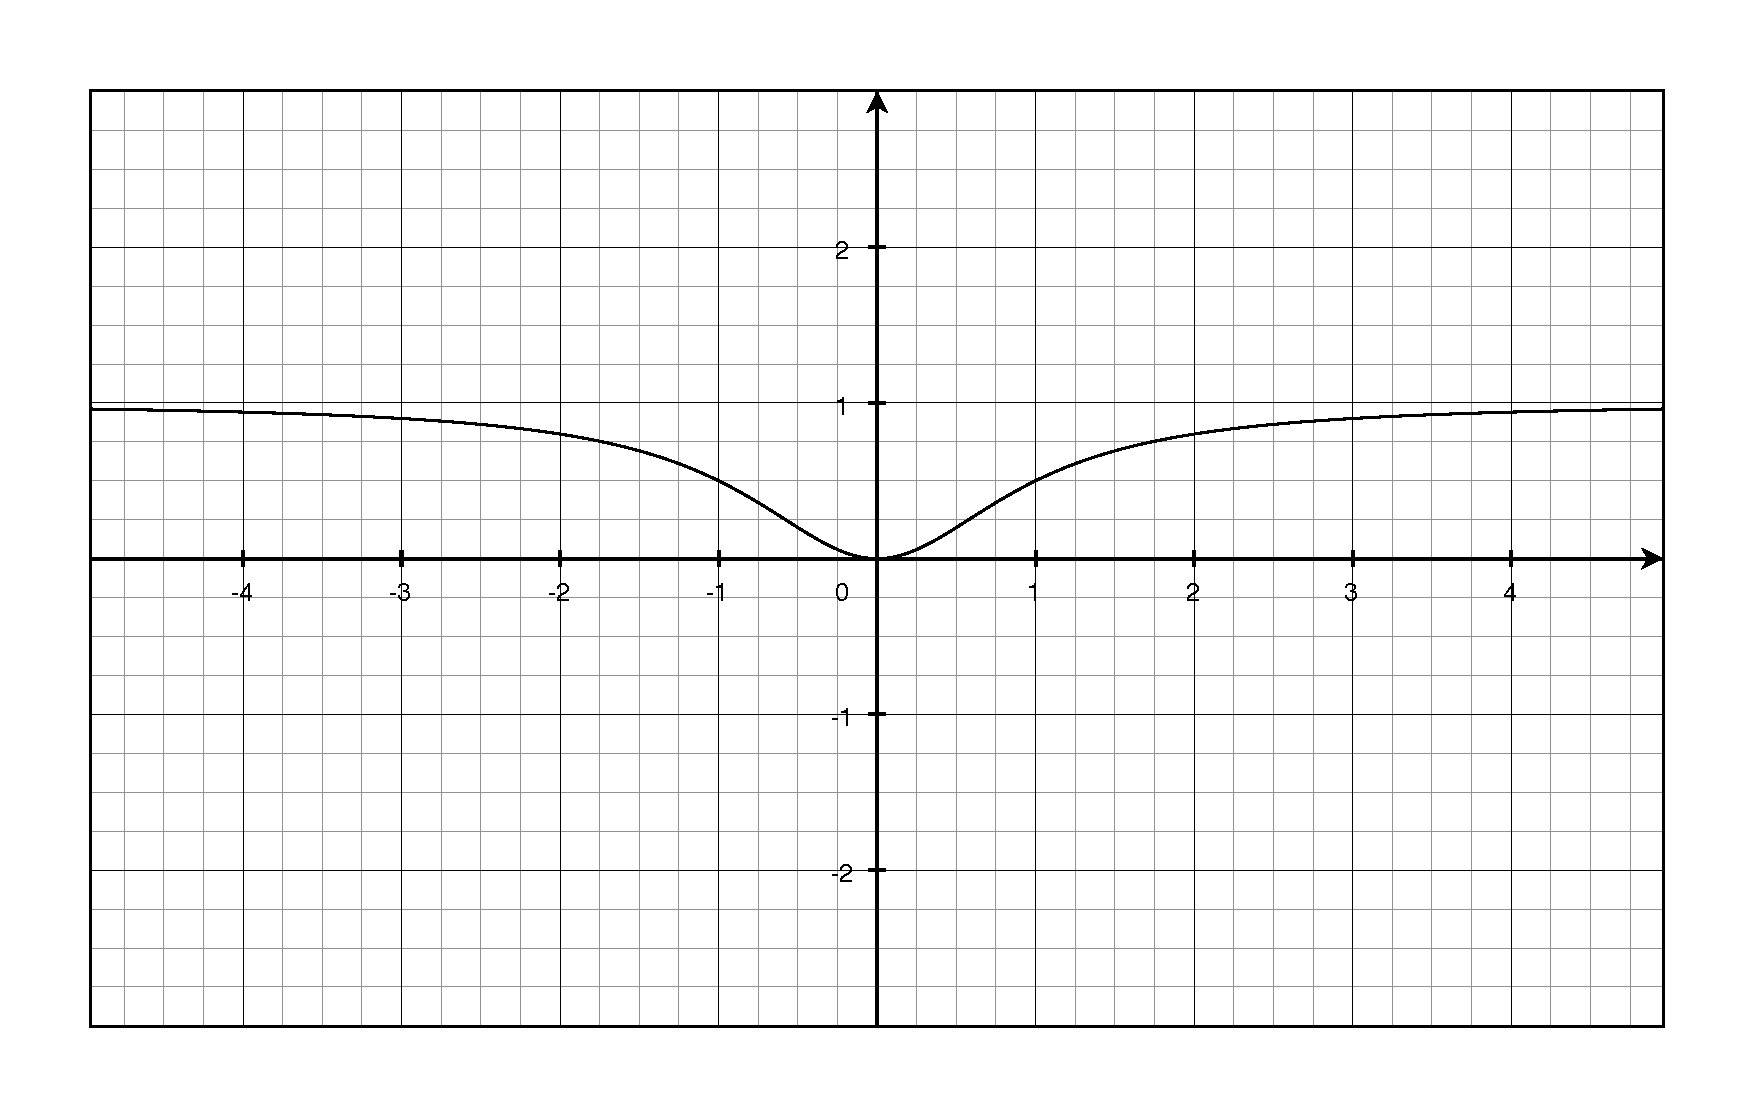
\includegraphics[scale=.3]{4.7.12.eps}
  \caption*{Question 12: $f(\theta) = \frac{\theta^2}{\theta^2 + 1}$}
\end{figure}


\item[16]
\begin{align*}
  f(z) &= z \sqrt{z + 1} \\
  f'(z) &= \frac{3z + 2}{2 \sqrt{z + 1}} \\
  f''(z) &=  \frac{3z + 4}{4 (z + 1)^{3/2}} \\
\end{align*}

Critical Numbers:
\begin{align*}
  3z + 2 &= 0 \\
  z &= -\frac{2}{3} \\
\end{align*}

Inflection Points:
\begin{align*}
  3z + 4 &= 0 \\
  z &= - \frac{4}{3} \\
\end{align*}
$-\frac{4}{3}$ is not in the range, so there aren't any inflection points.

\begin{itemize*}
  \item Increasing: $\left[- \frac{3}{2}, \infty \right)$
  \item Concave Up: everywhere
\end{itemize*}

\begin{figure}[H]
  \centering
  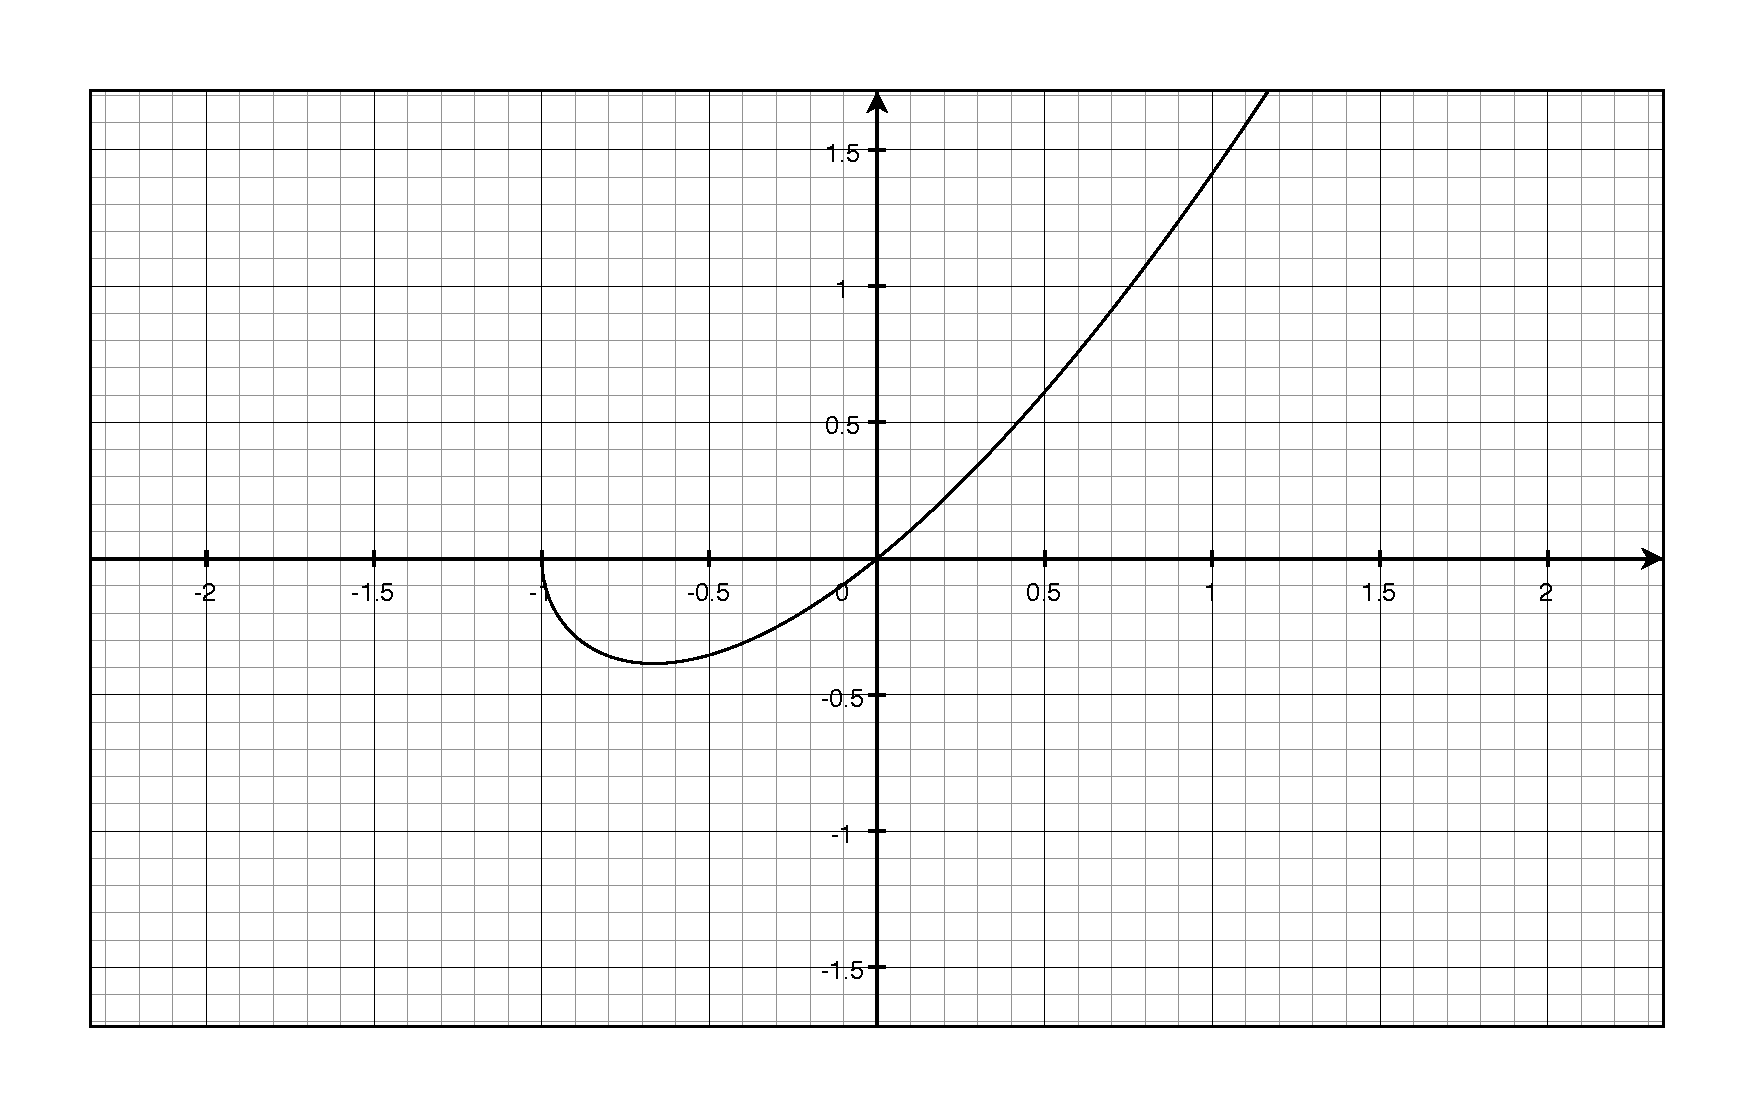
\includegraphics[scale=.3]{4.7.16.eps}
  \caption*{Question 16: $f(z) = z \sqrt{z + 1}$}
\end{figure}

\end{description}

\section{Section 4.8}

\begin{description}
\item[5]
\begin{align*}
  H(s) &= s^2 + 3s - 1 \\
  H'(s) &= 2s + 3 \\
\\
  rate_{avg} &= \frac{3 - (-1)}{4} = 1 \\
\\
  2s + 3 &= 1 \\
  2s &= -2 \\
  s &= -1 \\
\end{align*}

\item[6]
\begin{align*}
  F(x) &= \frac{x^3}{3} \text{; } [-2, 2] \\
  F'(x) &= x^2 \\
\\
  rate_{avg} &= \frac{4}{3} \\
\\
  x^2 &= \frac{4}{3} \\
  x &= \pm \frac{2}{\sqrt{3}} \\
\end{align*}

\item[7]
\begin{align*}
  f(z) &= \frac{1}{3} (z^3 + z - 4) \\
  f'(z) &= z^2 + \frac{1}{3} \\ \\
\\
  rate_{avg} &= \frac{2 - (-2)}{3} = \frac{4}{3} \\
\\
  z^2 + \frac{1}{3} &= \frac{4}{3} \\
  z &= \pm 1 \\
\end{align*}

\item[8]
The Mean Value Theorem doesn't apply because $F(1)$ is not defined.

\item[9]
\begin{align*}
  h(x) &= \frac{x}{x - 3} \text{; } [0, 2]\\
  h'(x) &= \frac{-3}{(x - 3)^2} \\
\\
  rate_{avg} &= -1 \\
\\
  \frac{-3}{(x - 3)^2} &= -1 \\
  x &= 3 - \sqrt{3} \\
\end{align*}

\item[10]
The Mean Value Theorem doesn't apply because $f(3)$ is not defined.

\item[13]
\begin{align*}
  g(x) &= x^{5/3} \\
  g'(x) &= \frac{5}{3} x^{2/3} \\
\\
  rate_{avg} &= \frac{1 - (0)}{1} = 1 \\
\\
  \frac{5}{3} x^{2/3} &= 1 \\
  x &= \sqrt[3] { \frac{9}{25} } \\
\end{align*}
 
\item[14]
\begin{align*}
  g(x) &= x^{5/3} \\
  g'(x) &= \frac{5}{3} x^{2/3} \\
\\
  rate_{avg} &= \frac{1 - (-1)}{2} = 1 \\
\\
  \frac{5}{3} x^{2/3} &= 1 \\
  x &= \sqrt[3] { \frac{9}{25} } \\
\end{align*}

\item[18]
The Mean Value Theorem doesn't apply because $f(0)$ is not defined.

\item[19]
\begin{align*}
  f(x) &= x + \frac{1}{x} \\
  g'(x) &= 1 - \frac{1}{x^2} \\
\\
  rate_{avg} &= \frac{5/2 - 2}{1} = \frac{1}{2} \\
\\
  1 - \frac{1}{x^2} &= \frac{1}{2} \\
  x &= \sqrt{2} \\ 
\end{align*}

\item[21] Let $d(t)$ be the function which gives the distance Johnny has travelled at time $t$ after the start time.
  Since Johnny travelled 112 miles in 2 hours, we know that:

\begin{align*}
  d(2) &= 112 \\
  rate_{avg} &= \frac{112 - 0}{2 - 0} = 56 \\
\end{align*}
 
From the Mean Value Theorem, there must be some time $t_0$ where $d'(t) = rate_{avg}$, so his instantaneous velocity must
have been 56 at some point.

\item[23]
The average rate of change over the interval seems to be about:
\[
  rate_{avg} = \frac{1 - 2}{8} = - \frac{1}{8}
\]

The points where the tangent has approximately this slope seem to be $x = \{2, 3.8, 7.8 \}$.

\end{description}

\else

\vspace{5 cm}

%% {\em A noble-minded person is different from others, but at peace with them.  A small-minded person is the same as
%%   others, but never at peace with them.}

%% {\em The noble-minded encourage what is beautiful in people and discuourage what is ugly in them.  Little people to just
%%   the opposite.}

{\em Unless you've been appointed to office, don't fuss and fret over the business of government.}
\vspace{.2 cm}

\hspace{1 cm} --Confucious

\fi

\end{document}

